% Chapter 2 is usually termed 'Related Work', 'State of the Art' or 'Fundamentals'. Here you will describe
% relevant technologies and standards related to your topic. What did other scientists propose regarding
% your topic? This chapter makes about 20-30 percent of the complete thesis.
%
% This section is intended to give an introduction about relevant terms, technologies
% and standards in the field of X. You do not have to explain common technologies such
% as HTML or XML.
%
% This section describes relevant technologies, starting with X followed by Y, concluding with Z.

\chapter{State of the Art\label{cha:state_of_the_art}}

There are two main standards/protocols that are used in this thesis and will be described in depth in this chapter: the HbbTV standard and the WebDriver protocol. Both are fairly new standards that have been defined within the last 5 years. Another important protocol for this work is the Chrome Remote Debugging protocol which is used by the automation driver to drive the WebDriver tests and to get data out of the HbbTV app. This thesis tries to connect these standards to allow interoperability between them to increase the level of integration to a wide variety of tools that has not been possible before.

\section{HbbTV\label{sec:hbbtv}}

% It's always a good idea to explain a technology or a system with a citation of a prominent
% source, such as a widely accepted technical book or a famous person or organization.

Television devices started to become connected to the internet already before HbbTV was invented. With the so called Set Top Boxes or Smart TV Sticks customers were able to connect the TV to an internet capable device that provided a content stream. Big companies like Google, Amazon or Apple offered such devices. The problem with this approach was that if a developer wanted to build an app he had to create this app for each individual platform. This is a really time-consuming and not scaleable process as the way you build apps for such platforms was extremely different. After game consoles like Sony PlayStation or Microsoft's xBox became internet connected devices too there even was another way to transform the normal TV to a Smart TV. It made it even more difficult for content providers to deploy their services to all TV platforms.

With the open ETSI standard called HbbTV a new way was build to create digital applications for broadcasters and content providers that runs on every TV supporting that standard. It \textit{''is a globally initiative technology mainly developed by industry leaders''} \cite{zte}. The standard itself introduces only a handful technical components and is mainly based on existing standards. HbbTV applications are HTML web pages with additional features that enable certain interaction between broadcast and broadband. It is sometimes referred to as Hybrid Television since the TV device receives data from both of these sources in parallel. This means that from a running broadcast stream it allows customers to open apps that provide additional content to the image on the screen. From that you can start even more applications that provide different content in non linear fashion. We have to differentiate here between two different types of apps. There are broadcast-independent applications that are not connected to any broadcast service and are downloaded and accessed via broadband. The other type are broadcast-related applications that can be opened when a certain broadcast service is used. They can start automatically or explicitly upon user request. The advantage of HbbTV here is the independence to the used device. Content providers can build and deploy apps which can be used by any device if the standard is supported.

If a consumer is equipped with an HbbTV supported Smart TV he will usually see a small image somewhere on the screen that offers to press the red button on the remote control. Pressing it triggers an event within the app that opens the HbbTV application. Once the user switches the channel the same happens again with a different app. Depending on the broadcaster each broadcast signal contains a small AIT package that contains main information like application ID, version, autostart state and application URL of the HbbTV app. Figure \ref{fig:app_delivery} demonstrates the workflow of this process.

\begin{figure}[htb]
  \centering
  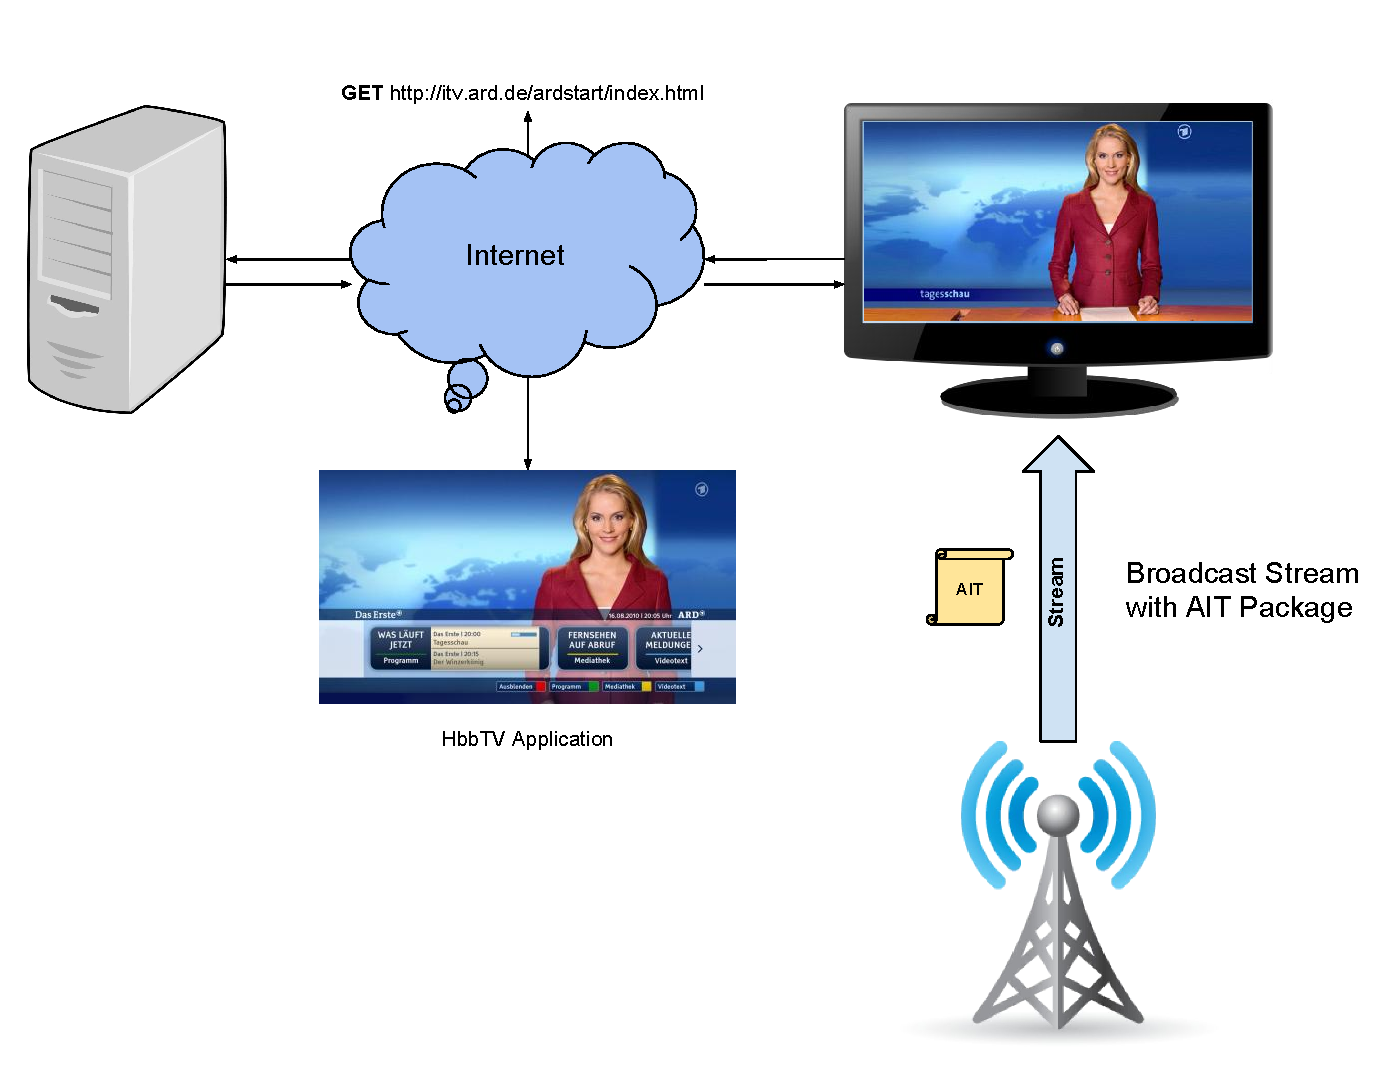
\includegraphics[width=15cm]{app_delivery.pdf}\\
  \caption{App delivery workflow of HbbTV applications}\label{fig:app_delivery}
\end{figure}

Depending on the autostart information within the AIT package the app either starts automatically as soon as the broadcast stream starts or only when the user pushes the red button. Most HbbTV applications these days use the autostart feature to display a small indicaticator image to show that an HbbTV app is available to use. Once the app opens, it either takes up only some part of the screen or fulfills the whole display. In general though the broadcast stream is never getting disrupted as the application only acts as an additional service to it.

After the first specification was released in 2010 by the \textit{''HbbTV forum and published by ETSI in the specification TS 102 796''} \cite{evolution} initiators reached out to CE manufactures to get it implemented in the next generation of TVs. Since then the number of Smart TVs with HbbTV support has increased drastically with more than 43 million devices sold and over 300 apps deployed in 25 countries\footnote{Source: \url{https://www.hbbtv.org/news-events/hbbtv-ibc-2016-services-and-devices/}} \footnote{A complete list of all countries can be found in Listing \ref{hbbtvdeployed} in the annex section}. Alone in Germany there are over 120 HbbTV supported channels\footnote{Source: \url{https://trifinite.org/hbbtv/trifinite_hbbtv_channel_list.html}} generating roughly 320 million hits monthly\footnote{Source: \url{https://goo.gl/eg8Sfs}}.

Almost two years later a new specification was released (HbbTV 1.5) that added support for MPEG DASH and MPEG CENC. MPEG DASH is an ISO standard for adaptive streaming of IP videos. Depending on the users bandwidth and CPU processing power it ensures continuous playback and helps to improve the stream experience in general by monitoring the CPU utilization and/or buffer status. If e.g. for any reason the user looses bandwidth the player is able to lower the quality of the video so that it still can be played without disruption. Due to support issues not many HbbTV apps use DASH these days. Most videos are still loaded in a progressive way. The MPEG CENC on the other side helps with common encryption for ISO based media format files and MPEG-2 transport streams. As a content provider using this feature you only have to encrypt your video once. The user then has to decrypt it by getting the key from one of many DRM systems.

The HbbTV 1.5 standard is supported by the majority of devices these days, however many CE manufactures already are about to support the latest HbbTV spec version 2 with their new devices on the market. It introduces a lot of new features and supports more web technology standards. While previous HbbTV apps only work with a version of CE-HTML which is an XHTML-based standard specifically for consumer electronic devices on UPnP networks, the latest specification supports HTML5, CSS3 and Web Sockets. Another new feature is the ability for synchronization of audio, video and data streams that enables the consumer to watch a certain broadcast stream while listening on the audio via broadband. This opens a wide variety of use cases like services for simultaneous translations of videos. It can be combined with the new introduced Second Screen Integration for smartphones and tablets which allows starting broadcast streams from your personal handheld on the TV. Due to its duplex communication ability it allows to also start videos from your HbbTV app on your mobile device. This works with multiple devices and also provides a lot of opportunities for e.g. gaming applications where phones can be used as remote controls. In the video area the specifications will support new streaming formats like HEVC, also known as H.265 and MPEG-H Part 2, DASH for DVB or push-on-demand where users are able to download certain videos on a local storage to watch them later if desired.

It is worth mentioning that version 2 of the spec was never really released by ETSI. It got surpassed by version 2.0.1 which fixed unclear specifications and removed some errors. It also shipped some additional specifications that were required to adapt the standard in Italy and United Kingdom who have decided to move from a similar standard called MHP to HbbTV. These specifications define additional caching rules for HTTP/1.1, more details on higher display resolution and other technologies that were defined in MHP.

An additional standard to HbbTV was released by ETSI shortly after HbbTV version 2. This standard is called Application Discovery over Broadband and is not part of the actual HbbTV specification. However it adds an important addition to HbbTV that is used if cable service providers block the AIT of the broadcast stream. These providers have a different idea of interactive TV services and usually want to promote their own platform. Once the AIT package is blocked the HbbTV application can't be loaded by the TV anymore since information about application ID and URL are missing. Application Discovery over Broadband is a workaround to solve this problem.

\begin{figure}[htb]
  \centering
  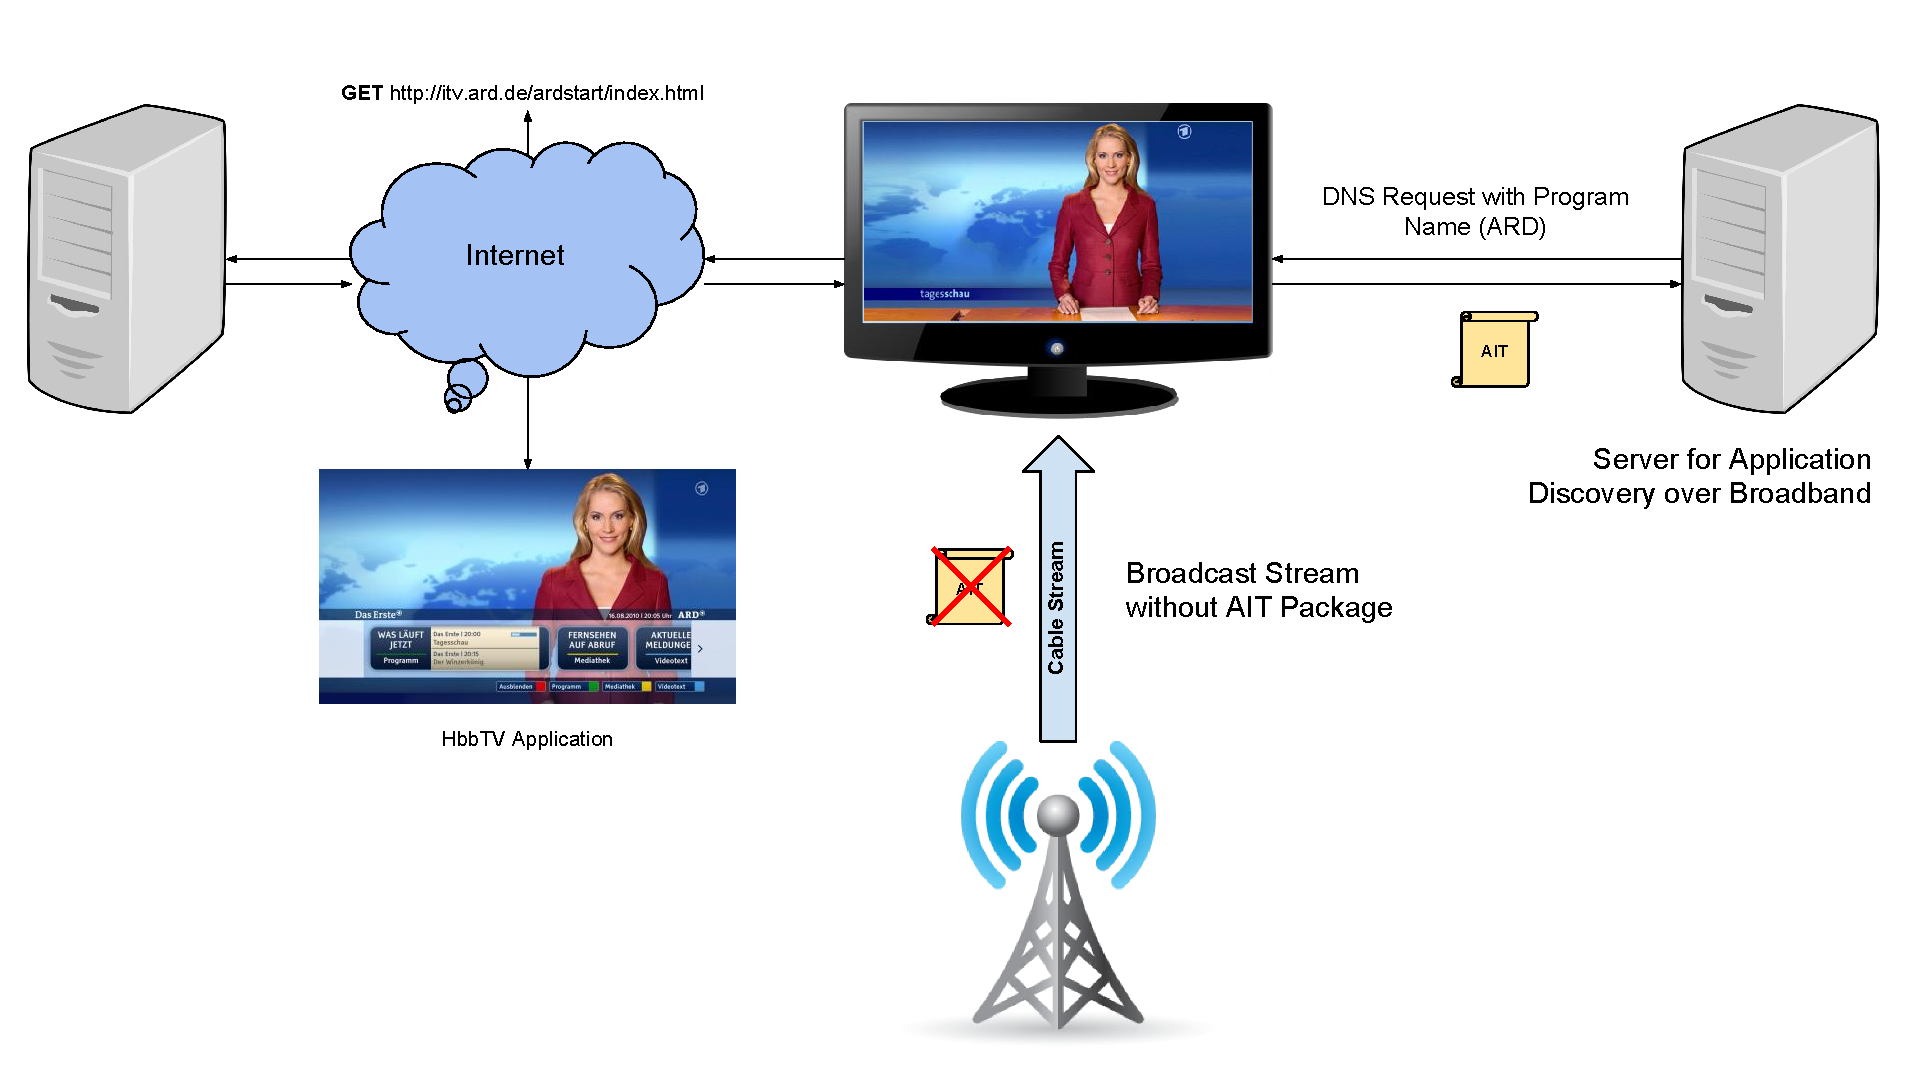
\includegraphics[width=15cm]{application_discovery_over_broadband.pdf}\\
  \caption{App delivery workflow of HbbTV applications over broadband discovery}\label{fig:application_discovery_over_broadband}
\end{figure}

As described in figure \ref{fig:application_discovery_over_broadband} the TV gets the AIT package from a dedicated server based on the program name. Each broadcaster usually has their own DNS root server and an own AIT server. However there is one main HbbTV DNS root server which routes the DNS request from the TV to the server of the broadcaster.

Pay, cable, IPTV or Sat-Platform operators as mentioned above sometimes provide instead of HbbTV their own service apps with a custom GUI. They usually require to use some sort of additional hardware which don't support HbbTV. Even though the TV is connected to the internet and supports the standard it is still not possible to open up an HbbTV application. As solution for this problem the consortium around the standard invented Operator Apps which allows connecting operator and HbbTV applications on one Smart TV. The idea is that the user can switch between both worlds as a functionality within the TV. Anyone who has a contract with the TV manufacture can become an operator. Each operator app has to authenticate to the TV to avoid abuse. Unlike HbbTV applications an operator app can run in the background at all times and can display messages on the display as well as overwrite key functions like \textit{''P+''} or \textit{''P-''}. They usually open by pressing \textit{''EPG''} or \textit{''Menu''}. In the specification of operator apps which is part of HbbTV version 2 the consortium emphasized that operator and HbbTV apps can live seamlessly together.

Looking back at the standard that was first specified 7 ago HbbTV has taken a very interesting development. From being able to show more than a digital and interactive teletext to supporting HTML5 and Second Screen it became quite comprehensive. This enables broadcasters to use this service in a variety of ways.

\subsection{Example Applications And Use Cases}

All these features allow broadcasters to implement not only an additional content outlet but also to create tailored advertisement strategies to a specified audience with methods like geo targeting or targeted advertisement. Geotargeting can be used in HbbTV applications by leveraging a users IP address in order show regional products or services. Combined with a broadcast stream it enables interesting opportunities. In an advertisement campaign launched by Germans private broadcaster RTL they promoted a pharmaceutical product with help of an HbbTV app. The pharmaceutical \textit{''Wick Medinait''} was advertised along with a banner that showed the regional weather forecast. It had the effect that the HbbTV app banner supported the TV spot so that it increased the impact of the advertisement itself.

\begin{figure}[htb]
  \centering
  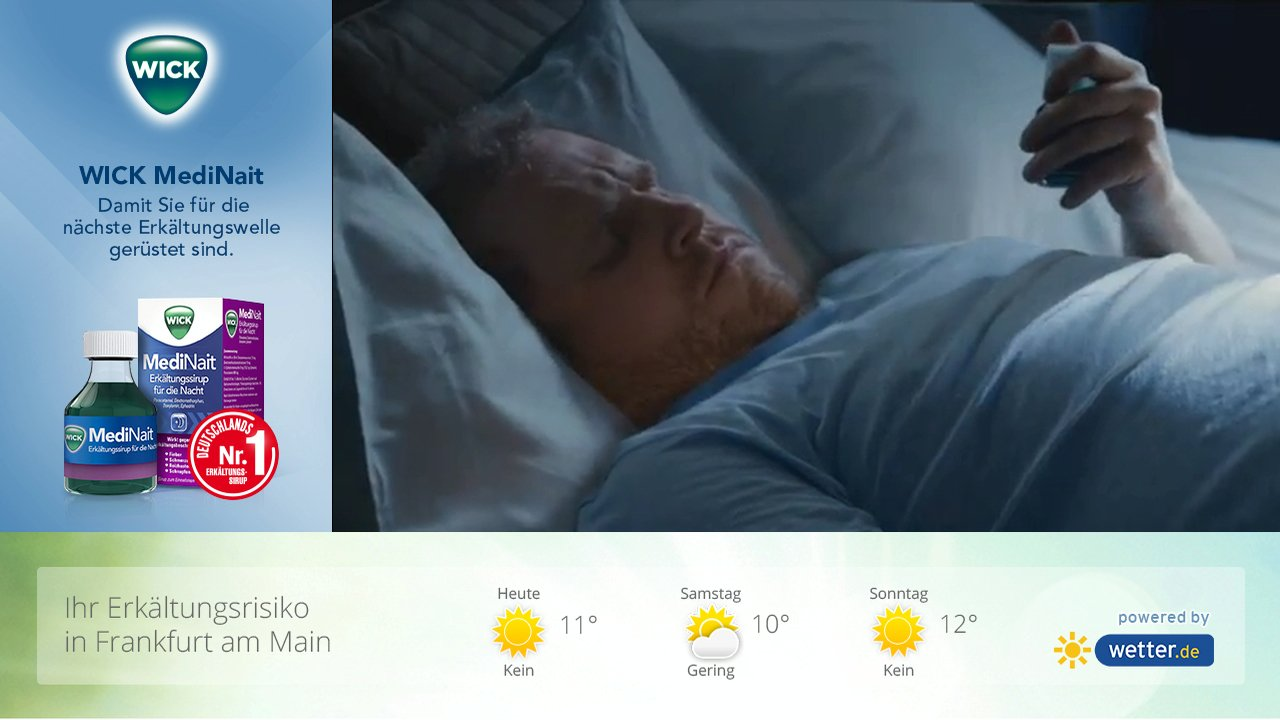
\includegraphics[width=10cm]{geotargeting.jpg}\\
  \caption{
    Use case of geo targeting via HbbTV\\
    {\tiny Image Source: https://goo.gl/rab8XD}
  }
  \label{fig:geotargeting}
\end{figure}

This is also called as Addressable TV advertising. It \textit{''enable[s] advertisers to selectively segment TV audiences and serve different ads or ad pods (groups of ads) within a common program or navigation screen. Segmentation can occur at geographic, demographic, behavioral and (in some cases) self-selected individual household levels [...]''}\cite{adrTV}.

Another interesting use case outside of advertisement is content authoring of HbbTV applications. Usually an HbbTV application is a custom web app that is build to serve a specific content for a service or show. Once you want to promote a new service or show it requires to build a new app with new content. This takes time and costs money. A solution to this problem was adapted from the web. By using a Content Management System (CMS), like Wordpress\footnote{\url{https://wordpress.org/}}, broadcasters can create or modify the content of their apps using a simple web interface.

\begin{figure}[htb]
  \centering
  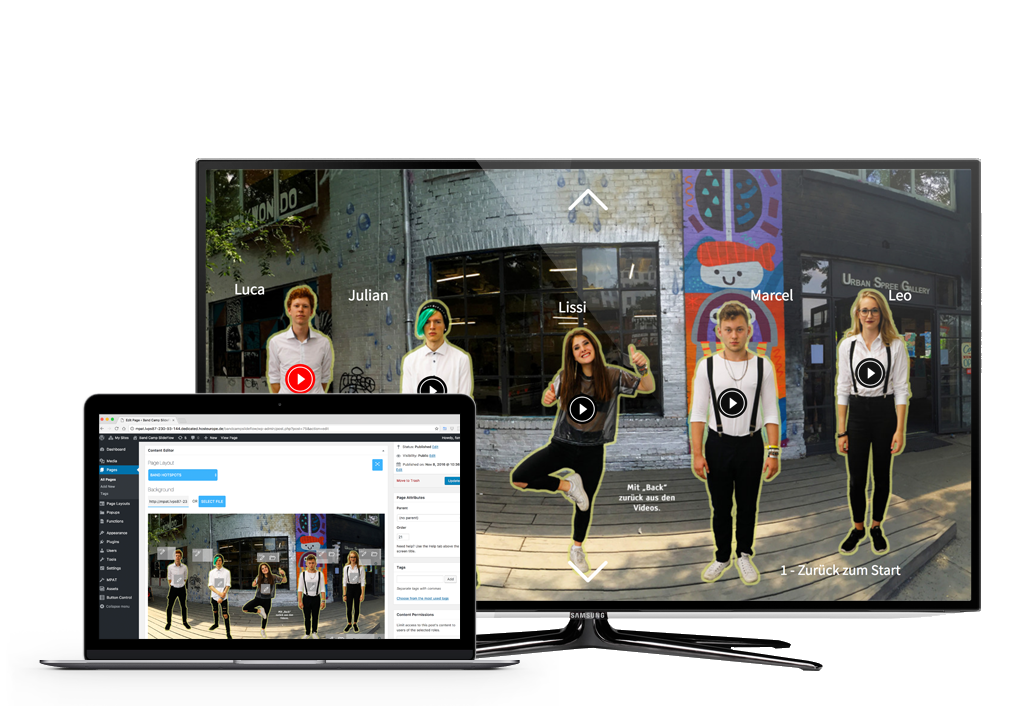
\includegraphics[width=10cm]{mpat.png}\\
  \caption{
    Modifying HbbTV content via a web interface
  }
  \label{fig:mpat}
\end{figure}

Figure \ref{fig:mpat} shows how this looks like with a tool called MPAT\footnote{\url{https://www.fokus.fraunhofer.de/en/fame/project/mpat}}, a project that was funded by the European Union and developed and led by Fraunhofer Fokus. It uses Wordpress as CMS to enable authors to modify content, look or functionality of an HbbTV app. Thanks to its plug\&play functionality the tool can easily add new features like Chat and Video or Image Galleries without requiring someone to implement it. With that it reduces the risk of unexpected behavior as these plugins are already tested against common Smart TV devices.

\subsection{HbbTV Runtime Environment\label{sec:hbbtvruntimeenvironment}}

The Runtime Environment of an HbbTV application is formed by the browser and an Application Manager who \textit{''evaluates the AIT to control the lifecycle for an interactive application''}\cite{hbbtv15}. The browser on the other side, which is in many cases a clone of an already existing web browser with a subset of supported features, is responsible to render the HbbTV app. The TV receives an AIT package, an A/V signal as well as application data and stream events from the broadcast stream. While the A/V stream is processed like a standard non-hybrid DVB stream it still can provide some information like channel list or tuning functions to the runtime environment. Furthermore receives the runtime environment the application data and event streams from the object carousel using a DSM-CC client which is a toolkit defined in the MPEG-2 standard that provides a control channel to access the broadcast stream and push data to the Application Manager.

\begin{figure}[htb]
  \centering
  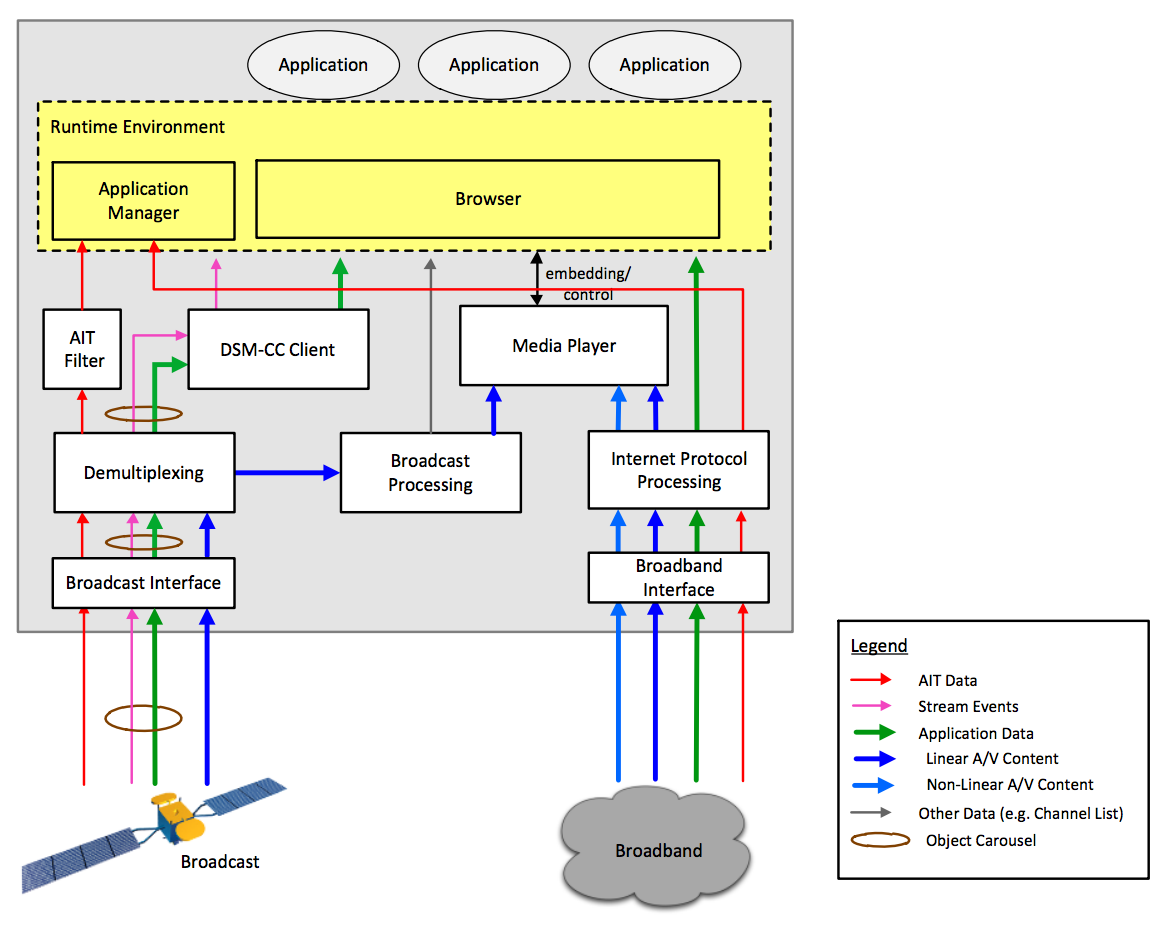
\includegraphics[width=15cm]{app_env.png}\\
  \caption{
    Functional components of a hybrid terminal
  }
  \label{fig:app_env}
\end{figure}

In order to allow the HbbTV app to embed the running broadcast stream within the application as a video, the Media Player component is required which receives that data after the broadcast stream was processed. It can also receive A/V content from the broadband source in linear or non linear form.

As described in section \ref{sec:hbbtv} once the HbbTV application is loaded via broadband stream, it starts either directly by the end-user by pressing a dedicated button on the remote control, in response to an event stream or by an already running application, e.g. when the user wants to open an application within the application. With HbbTV version 2 it became also possible to start the app with a companion screen. However it is often the case that the app is a broadcast related autostart application which displays a \textit{''Red Button''} notification to inform the user that an application is available. These are called \textit{''Red Button''} applications. To not disrupt the video stream they only show something like a small image and leave the rest of the screen transparent using CSS. This has been agreed in a guideline to not annoy the viewer with undesired overlays and to allow a uniform experience for the application start. If no action is taken by the user this indicator disappears again. Since radio services don't have this indicator, because they don't use the video channel, the full user interface will be displayed. Some applications like digital teletext apps are not run with autostart enabled. They have to be specifically triggered by the user without notification, in this case using the teletext button on the remote. Triggered one time it starts the digital teletext which is an HbbTV based application. If triggered twice it closes this app and starts the standard old-fashioned teletext. By pushing the button for the third time it closes also that.

HbbTV apps are not only tied to a specific broadcaster. The so called broadcast-independent applications \textit{''can be electronic programme guides (EPGs) or “TV editions” of existing web services such as flickr, YouTube and very many more that may be provided by the big brands as well as on a regional level or even by individuals.''}\cite{biapps}

\subsection{Development of HbbTV Applications\label{sec:devofhbbtv}}

As mentioned in \ref{sec:hbbtv} HbbTV applications are written in CE-HTML which is an XHTML based standard to build web pages for consumer electronics like televisions. With the release of HbbTV version 2 support for HTML5 was added which allows developers to use the latest web technologies in their apps. Until the majority of devices have support for that, apps will be still delivered in the CE-HTML format. Per specification the doctype of the document needs to be either XHTML 1.0 strict or has to have an HbbTV specific declaration which is

\vspace{1cm}
\begin{listing}[H]
\begin{minted}[mathescape, linenos, numbersep=8pt, gobble=0, framesep=2mm]{html}
<?xml version="1.0" encoding="UTF-8" ?>
<!DOCTYPE html PUBLIC "-//HbbTV//1.1.1//EN"
  "http://www.hbbtv.org/dtd/HbbTV-1.1.1.dtd"
>
<html xmlns="http://www.w3.org/1999/xhtml">
  <head>
    <meta http-equiv="Content-Type"
          content="application/vnd.hbbtv.xml+xhtml; utf-8"
    />
\end{minted}
\caption{Beginning of an HbbTV document}
\label{lst:doctype}
\end{listing}
\vspace{0.5cm}

Also the document needs to contain an XML declaration at the beginning of the document as well as a namespace definition in the HTML tag. This is required so that the device can properly interpret the document as CE-HTML. In addition to that the page needs to be served with an \textit{''application/vnd.hbbtv.xml+xhtml''} content type otherwise the app is going to be ignored by the television. The browser window has a fixed size of 1280x720 pixel and therefor fits perfectly in full screen on a 16:9 device. With embedded objects the developer can access APIs that are defined by the Open IPTV Forum in the HbbTV spec to receive TV capabilities and configuration as well as access the application manager. It extracts information out of the AIT packages such as lifecycle of the app or the autostart flag. APIs are available for configuration and settings, download manager and content download as well as parental access control and scheduled recordings. However most HbbTV apps these days only need the following embedded objects:

\vspace{1cm}
\begin{listing}[H]
\begin{minted}[mathescape, linenos, numbersep=8pt, gobble=0, framesep=2mm]{html}
<object type="application/oipfApplicationManager" id="oipfAppMan" />
<object type="application/oipfConfiguration" id="oipfConfig" />
\end{minted}
\caption{Embedded Objects used to access HbbTV APIs}
\label{lst:embeddedObjects}
\end{listing}
\vspace{0.5cm}

Using the DOM node id developers can query the element and access the API. This usally happens on the \textit{''onLoad''} event that gets triggered onced all DOM elements and JavaScript files are loaded. The event callback then executes some sort of initialization method that loads the applications and shows it on the screen.

\vspace{1cm}
\begin{listing}[H]
\begin{minted}[mathescape, linenos, numbersep=8pt, gobble=0, framesep=2mm]{javascript}
var oipf = document.getElementById(appMan);
var app = oipf.getOwnerApplication(document);
app.show();
\end{minted}
\caption{HbbTV App initialization}
\label{lst:loadApp}
\end{listing}
\vspace{0.5cm}

The only input device for HbbTV web apps is the remote control. Within the initialization process an event listener is registered on the window global object that gets triggered on keydown events. Depending on the event key code the app executes different actions and allows navigating through the app.

Since uploading changes to a production server is inefficient and time-consuming people have developed some tools to improve the development environments of HbbTV app developers. There is a Firefox plugin that emulates an CE-HTML-like environment in the browser called FireHbbTV\footnote{\url{https://addons.mozilla.org/en-US/firefox/addon/firehbbtv/}}. It simulates the TV Remote control using the standard keyboard, displays the safe-area margin as well as supports most of the HbbTV specific APIs. Another popular tool is the Opera TV Emulator\footnote{\url{http://www.operasoftware.com/products/tv/tv-developer-tools}}, a virtual machine that emulates an Opera SmartTV environment. With that you can have your app being served on your local machine and easily access it using these tools. However even though these are helpful tools \textit{''they don't offer the full capacities and facilities that a certified HbbTV device will provide.''} \cite{hbbtvenv}. Therefor many developers tend to build their apps directly on the TV with some sort of debug overlay that prints custom debug messages.

\subsection{Available test solutions\label{sec:availabletestsolutions}}

Most of the standard static code analysis tools like JavaScript or CSS linters also apply for HbbTV app development. These tools ensure that the code can be parsed by the TV device. Specifically for HbbTV apps the \textit{''Institut für Rundfunktechnik GmbH''} authored a validator\footnote{\url{http://hbbtv-live.irt.de/validator}} that checks for common pitfalls. It not only warns you if you serve the app with a wrong content-type it also makes sure that other specifications are met like having the right doctype or required XML namespace attributes set. However these helpers can only detect obvious issues that are relevant to all HbbTV devices. Problems that only appear on TVs from certain manufactures can not be found with these kind of tools. It usually requires manual work which ends up being very tedious and expensive. There are some companies that tried to solve this problem.

A Czech company called Suitest has developed a system to run e2e tests based on a web GUI on arbitrary devices either in a remote office or in a local environment. It allows to run these tests in parallel and provides a comprehensive report about the test result over time. The GUI allows their user to simply click together one or multiple test scenarios with common actions like: open the app via URL, press a button on the remote and assert that a certain element contains a certain property. Every aspect of your test can be separated into sub steps and reused in other tests. The main idea is that you don't need any coding skills to put together a test. Figure \ref{fig:suitest} shows how simple the GUI looks like and how tests are being put together.

\begin{figure}[htb]
  \centering
  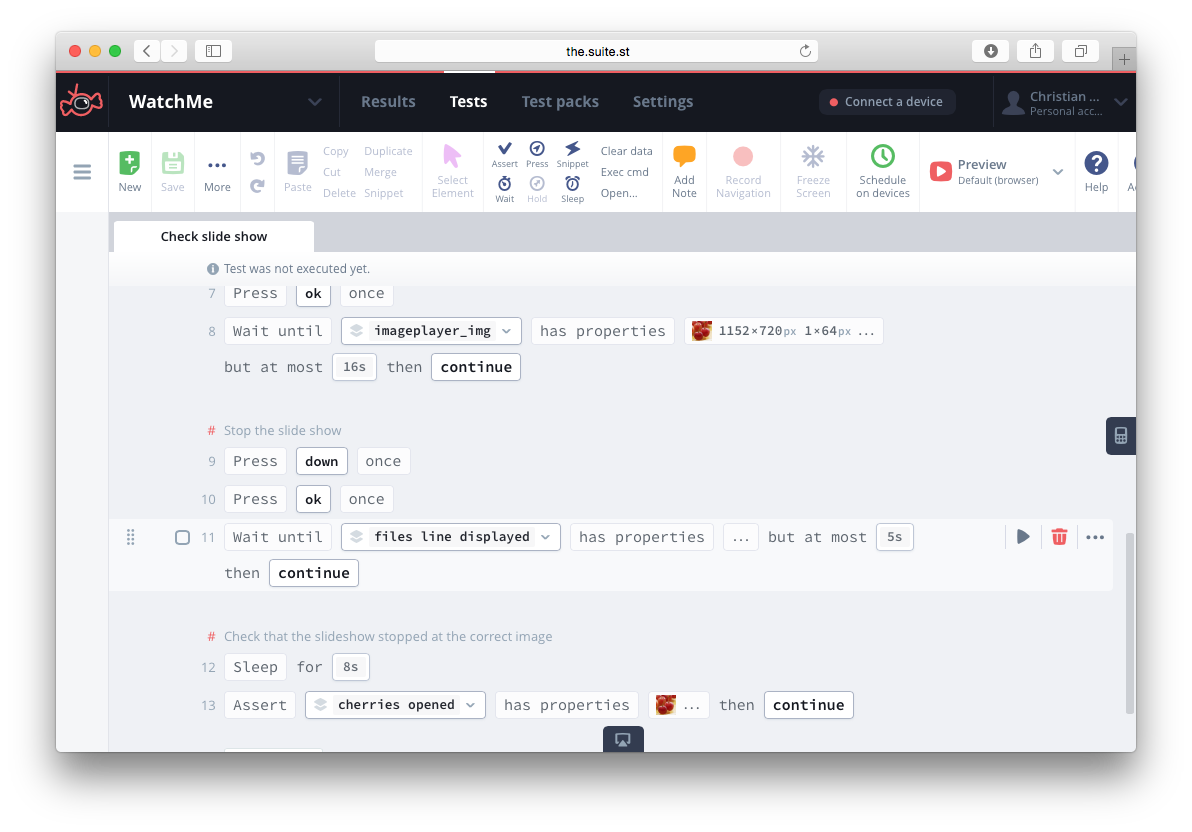
\includegraphics[width=15cm]{suitest.png}\\
  \caption{Suitest Test Editor GUI}\label{fig:suitest}
\end{figure}

To gain access to the device the company provides a setup box that comes with infrared blasters in order to simulate remote control events. You can also inject a script into your HbbTV app to instrument either your browser or TV device to allow Suitest to run your tests. In case you don't own a targeted device Suitest provides a handful of devices from their own datacenter. It requires a paid plan though which starts with 156\euro{} up to 899\euro{}\footnote{\url{https://suite.st/pricing.html}}.

Another company providing an e2e test solution for HbbTV apps on Smart TVs is \textit{Eurofins Digital Testing}\footnote{\url{http://www.eurofins-digitaltesting.com/}}. Next to HbbTV applications they also offer multiple device types such as Set-Top Boxes, standard web-apps or mobile apps on tablets and phones. Their TestWizard Manager\footnote{\url{http://www.eurofins-digitaltesting.com/testwizard/infrastructure/}} controls a set of TestWizard Robots that contain a different variety of devices depending on the requirements of the application. Unlike Suitest the company offers a development tool called \textit{ScriptStudio} that allows customer to also write automated tests \textit{''without requirement for extensive knowledge of scripting languages''} \cite{scriptstudio}. Since other devices types that they offer for mobile and desktop can be tested via test automation scripts it is also possible to write e2e tests via Selenium and Appium. The company itself is with 22,000 employees way bigger than Suitest. They have a network of more than 200 laboratories and offer complete testing solutions not only for HbbTV but also for other key technologies and standards such as DVB or DASH.

\subsection{Web Platform Tests}

Within the last decade many organizations including the W3C tried to build standards around technologies that we use everyday. Even though these specifications were adapted by developers and companies there was still a lack of conformance, quality of implementation, performance and interoperability. In 2013 the W3C launched \textit{''an unprecedented effort to scale up its test offering''} \cite{w3ctesting} in which they tried to improve the test infrastructure and documentation around all web standards that are defined by them. By streamlining the contribution and reviewing processes they simplified the way how everyone can be involved in defining and testing a standard. They published their tests and made them accessible for everyone so that anybody was able to get a clear picture of which web features are supported in whatever application they are testing. With that every browser vendor was able to make sure that its browser is working according to the spec. They became the major contributor for writing and maintaining the tests. However the W3C also encouraged every developer to be involved in this endeavor by starting a movement called \textit{''Test the Web Forward''}\footnote{\url{http://testthewebforward.org/}}. This was one of major reasons why standards like HTML5 and other technologies that are part of the HbbTV specification got reliable implemented in many browsers and platforms.

The HbbTV specification which was defined within the European Telecommunications Standards Institute did something similar to ensure that TV manufactures only sell devices that are complaint to the spec. This is important as \textit{''lean-back consumers have zero patience meaning any malfunction in the chain will significantly reduce engagement and impact and may even result in viewers switching to another service''} \cite{hbbtvtesting}. In case of an update in the standard the association has to make sure that older applications are interoperable with forthcoming receivers and can coexist with them especially since devices are not easily updated by the consumer. Therefor they defined a receiver specification and a device and application conformance that sets certain guidelines and restriction to manufactures and developers to fulfill the standard and enforce on a common sense. Similar to the W3C a test suite\footnote{\url{https://www.hbbtv.org/resource-library/\#testing-information-and-support}} is provided to manufactures \textit{''to certify their own devices or have their devices certified by an HbbTV Registered Test Centre.''} \cite{hbbtvtesting}. Once they are certified they can use the official HbbTV logo for their device products as proof for compliance to the spec.

\section{Test Automation\label{sec:testautomation}}

There are a lot of different ways on how to test software. Depending on its type and the scope of the tested functionality there are multiple testing methods that can be applied. From unit testing, that only covers individual software components and code segments, to load testing, which makes sure that a specific performance metric is met, these methods are used at different stages of the development lifecycle. With test automation these testing methods can be executed with use of special software that controls the execution of tests and compares the actual state with a certain predicted outcome. This happens in an automated fashion so that the test itself is mostly triggered by a certain event (e.g. code changes) in a CI/CD like environment.

From the agile world where coding and testing are one process a concept developed by Mike Cohn became popular that describes how \textit{''an effective test automation strategy calls for automating tests at three levels: unit, service and UI''} \cite{testautomation}. It explains that \textit{''unit testing should be the foundation of a solid test automation strategy and as such represents the largest part of the pyramid''} \cite{unittesting}. On the other side user interface tests which are placed at the top of the pyramid should be as small as possible as they are brittle, error prone and time-consuming. However they simulate real user scenarios and ensure that the functionality is working on all levels, from database over the backend to the user interface. According to Googles philosophy \textit{''focus on the user and all else will follow''} you could convince someone that writing only e2e tests is a good idea even though it would object the test automation pyramid. Many developers follow this bad practice of having to many e2e tests (inverted pyramid or ice cream cone pattern) or a lot of unit and e2e tests but almost not integration/service level tests (hourglass pattern). A good rule of thumb here is splitting tests into 70\% unit tests, 20\% integration tests and 10\% e2e tests. Especially when working as an HbbTV app developer the desire to test apps directly on multiple TVs is high due to the high device fragmentation in the market.

Testing software from end to end is a hard problem to solve. It either requires manual work, which costs a lot of time, or engineering effort to automate this process. Over the last years the tech industry moved from manual QA to automated testing due to the \textit{''shift from Waterfall to Agile development''}\cite{shifttoautomated}. Software these days gets released in shorter cycles and feedback loops. Especially due to the growing popularity of DevOps, development and operations teams are no longer soiled and engineering work takes up the entire application lifecycle, from building the app to test and deployment. This allows not only to innovate for customers faster and adapt better to changes in market, it also forces you to increase the frequency and pace of releases in order to improve the product faster overall. Software has become \textit{''an integral component of every part of the business''} \cite{devops}. One fundamental practice in DevOps is Continuous Integration and Delivery. It improves the software quality by running automated tests on regular bases after code changes were committed. Once tests have passed, developers can automatically push their code to production with a high level of confidence that no regressions were introduced. This can only be accomplished with proper tooling. In order to test software from end to end a framework called Selenium has become the tool of choice for many developers.

\subsection{Selenium\label{sec:history}}

Selenium is a set of tools and libraries to automate mainly web browsers and mobile devices. It can interact with them to simulate user actions like click or inputs and assert certain states of web applications. These libraries are open source, available in almost any code language and are used to run e2e tests. It is supported by all the major browsers where each one provides some sort of automation driver that speaks the Selenium/WebDriver protocol. The communication is based on HTTP requests between an automation server and the client. Each test automation is coupled to a session id. Once a session is initiated you can communicate with the automation server via rest API. Such a server can be either a Selenium server or directly a browser automation driver. A Selenium server can be used to setup a grid of automation drivers to load balance requests based on its capabilities to a specific browser in the network. These browsers can be installed on different operating systems with different environments. It manages all initiated sessions and reroutes them accordingly. A browser automation driver can register itself as a single node to this hub server to make itself available for others to use. It allows to speed up the execution time by running tests on multiple browsers at the same time.

\begin{figure}[htb]
  \centering
  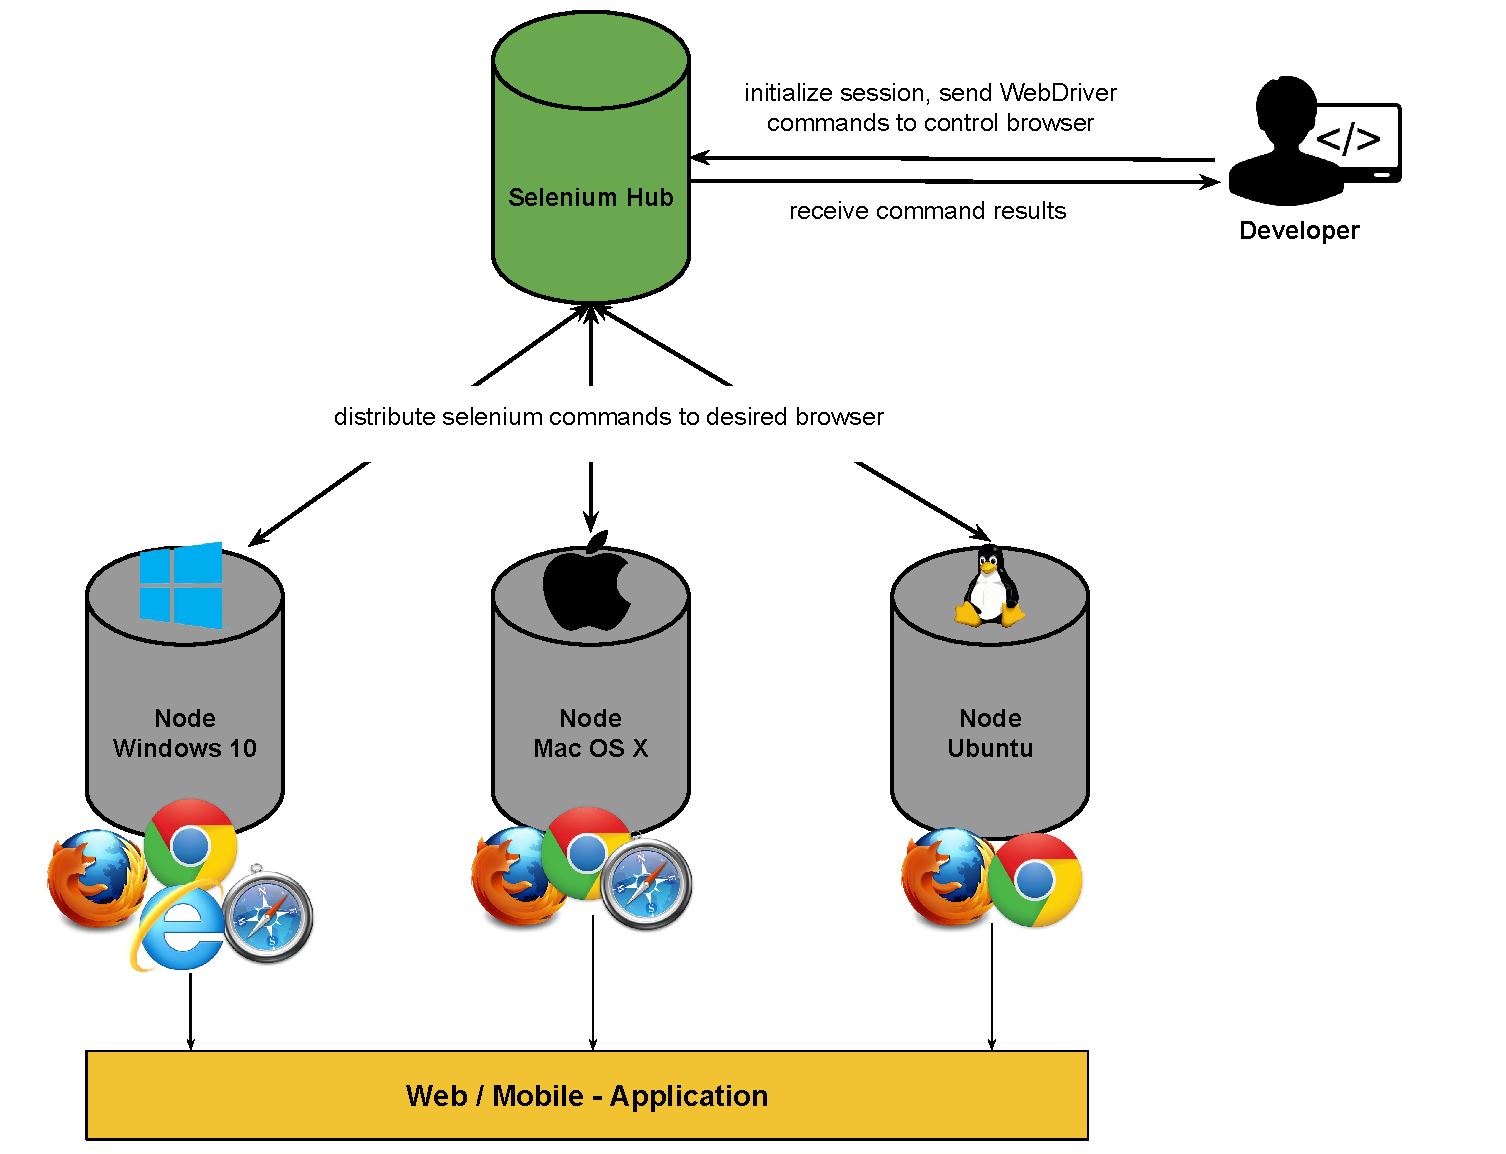
\includegraphics[width=15cm]{selenium.pdf}\\
  \caption{Concept Flow of a Selenium Grid}\label{fig:selenium}
\end{figure}

It is important to point out the difference between Selenium and WebDriver here. Selenium was developed in 2004 by Jason Huggins, an engineer at Thoughtworks\footnote{\url{https://www.thoughtworks.com}} who tried to build a tool to test web applications that require frequent testing. The tool was called \textit{JavaScript Test Runner}. It was able to interact with the web page in order to call certain actions on it. Due to the Same Origin Policy that was introduced by browser vendors to prevent JavaScript from accessing data from pages that are not within the same domain, Huggins and his team had to build a proxy server to overcome this. It injected a script to the web page to talk to the proxy server and therefor enable the interaction with the browser environment. This proxy server was released to the public as Selenium Remote Control and is the first version of Selenium. In 2007 Simon Stewart who was also working at Thoughtworks build another tool to run browser tests which he called WebDriver. His tool was not a proxy. It communicated with the browser directly to use its own engine for automation. In 2011 both tools got merged into one project that was called Selenium WebDriver (or Selenium 2.0). Over years it became the number one choice of developers for browser automation so that originators and the community around the project decided to make the Selenium protocol (also called JsonWireProtocol) a W3C standard. In 2016 this standard was released by the consortium as candidate recommendation after it was fully implemented in two major browsers (Firefox and IE). It was officially called WebDriver specification. Even though Selenium and WebDriver are referencing the same project and technology it still differs in some minor specification details. The Selenium project itself nowadays only contains the tools that can be used to run tests with WebDriver. Every part that was responsible to automate the browser became obsolete after all browser vendors stepped up to implement the automation engine directly into the browser.

\subsection{Appium\label{sec:appium}}

After the success of Selenium and the growing market of mobile devices and applications the demand for automating mobile phones increased more and more. Even though the big player in the market (Apple and Android) did provide tooling to create automated tests it still was time-consuming and cumbersome as both platforms forced developers to use their own platform specific technologies. With that it not only took twice as long to build the app since they had to be written in Java for Android and Objective-C for iOS respectively, they also had to be tested with two different frameworks. Appium aims to solve this problem by providing a cross platform solution for native and hybrid apps. It allows developers to write automated e2e tests on both platforms using the WebDriver protocol. It extends that protocol to introduce mobile specific actions like swipe or touch gestures to the developer. Moreover Appium supports hybrid applications as well which are mobile web apps that are wrapped within a tiny native container so that you can write one single app and deploy it for both platforms. With that it can also run a random web page on a browser on the mobile device. Since it leverages the native test automation frameworks it doesn't matter if you run your test on an emulator or simulator on your computer or a real device that is setup in a test lab. Since the WebDriver protocol is universal it doesn't require writing tests for Appium in a certain language. Similar to Selenium it is possible to write tests with any tool that supports the protocol. It also allows connecting to a Selenium Grid to not only have a browser but also a mobile grid available to use for automated tests.

\section{Chrome Remote Debugging Protocol\label{sec:remotedebuggingprotocol}}

As described in section \ref{fig:selenium} when Selenium merged with WebDriver they started to communicate with the browser directly in order to interact with the page. When the first automation driver for Google Chrome was released, it used an internal protocol called Chrome DevTools Protocol to instrument and debug the web page. By that time this protocol was mostly utilized to run the Chrome DevTools which is a developer tool to inspect the wepage and profile the underlying rendering engine called Chromium. The protocol is divided into a number of domains where each \textit{''domain defines a number of commands it supports and events it generates''} \cite{devtoolsprotocol}. If the user activates a flag\footnote{e.g. in Windows: chrome.exe $--$remote-debugging-port=9222} when starting the browser a TCP server is initiated and the API can get accessed via a WebSocket connection. This allows to remotely control the browser in almost any possible way. The protocol itself is comprehensive and allows besides receiving information about the state of the page a lot of debugging and profiling tools. Since it is part of WebKit which is the layout engine for many browsers - including Chrome (which uses a fork of WebKit called Blink), Safari or Opera - it gets utilized for debugging purposes in many web environments. Due to the number of already existing integrations (including Chrome DevTools) it almost makes it an universal protocol for automating a browser.
